\documentclass{cslthse-msc}
\usepackage[utf8]{inputenc}
\usepackage[english]{babel}
\usepackage{amsmath}
\usepackage{amsfonts}
\usepackage{amssymb}
\usepackage{amsthm}
%\usepackage{makeidx}
\usepackage{graphicx}
\usepackage[titletoc, header, page]{appendix}

\usepackage{hyperref}
\usepackage{pdfpages}

%\geometry{showframe}

\author{
	Flavius Gruian \\
	{\normalsize \href{mailto:Flavius.Gruian@cs.lth.se}{\texttt{Flavius.Gruian@cs.lth.se}}}
	\and
	Camilla Lekebjer \\
    {\normalsize \href{mailto:Camilla.Lekebjer@cs.lth.se}{\texttt{Camilla.Lekebjer@cs.lth.se}}}
}

\title{Formatting a Master's Thesis}
\subtitle{A {\LaTeX} class}
%\company{The Corporation AB LTD Inc}
\supervisors{John Deer, \href{mailto:jdeer@company.com}{\texttt{jdeer@company.com}}}{Don Jeer, \href{mailto:djeer@xy.lth.se}{\texttt{djeer@xy.lth.se}}}
%\supervisor{John Deer, \href{mailto:jdeer@company.com}{\texttt{jdeer@company.com}}}
\examiner{Jane Doe, \href{mailto:jane.doe@cs.lth.se}{\texttt{jane.doe@cs.lth.se}}}

\date{\today}
%\date{January 16, 2015}

\acknowledgements{
If you want to thank people, do it here, on a separate right-hand page. Both the U.S. \textit{acknowledgments} and the British \textit{acknowledgements} spellings are acceptable.

We would like to thank Lennart Andersson for his feedback on this template.
}

\theabstract{
This document describes the Master's Thesis format for the theses carried out at 
the Department of Computer Science, Lund University. 

Your abstract should capture, in English, the whole thesis with focus on the problem and solution in 150 words. It should be placed on a separate right-hand page, with an additional \textit{1cm} margin on both left and right. Avoid acronyms, footnotes, and references in the abstract if possible.

Leave a \textit{2cm} vertical space after the abstract and provide a few keywords relevant for your report. Use five to six words, of which at most two should be from the title.
}

\keywords{MSc, template, report, style, structure}

%% Only used to display font sizes
\makeatletter
\newcommand\thefontsize[1]{{#1 \f@size pt\par}}
\makeatother
%%%%%%%%%%


\begin{document}
\makefrontmatter
\chapter[Short on Formatting]{Formatting}
Avoid empty spaces between \textit{chapter}-\textit{section}, \textit{section}-\textit{sub-section}. For instance, a very brief summary of the chapter would be one way of bridging the chapter heading and the first section of that chapter.
\section{Page Size and Margins}
Use A4 paper, with the text margins given in Table \ref{tab:margins}.
\begin{table}[!hbt]
\centering
\caption{Text margins for A4.}\label{tab:margins}
\begin{tabular}{cc}
\hline
\textbf{margin} & \textbf{space} \\
\hline 
top &  3.0cm\\ 

bottom & 3.0cm \\ 
 
left (inside) & 2.5cm \\ 

right (outside) & 2.5cm \\ 

binding offset & 1.0cm \\ 
\hline 
\end{tabular} 
\end{table}

\section{Typeface and Font Sizes}
The fonts to use for the reports are \textbf{TeX Gyre Termes} (a \textbf{Times New Roman} clone) for serif fonts, \textsf{\textbf{TeX Gyre Heros}} (a \textsf{\textbf{Helvetica}} clone) for sans-serif fonts, and finally \texttt{\textbf{TeX Gyre Cursor}} (a \texttt{\textbf{Courier}} clone) as mono-space font. All these fonts are included with the TeXLive 2013 installation. Table \ref{tab:fonts} lists the most important text elements and the associated fonts.
\begin{table}[!hbt]
\caption{Font types, faces and sizes to be used.}\label{tab:fonts}

 \begin{tabular}{ l c c c}
\hline 
\textbf{Element} & \textbf{Face} & \textbf{Size}  & \textbf{\LaTeX size}  \\ 
\hline 
{\huge \textbf{Ch. label}} & {\huge \textbf{serif, bold}} & \thefontsize\huge & \verb+\huge+ \\ 
{\Huge \textbf{Chapter}} & {\Huge \textbf{serif, bold}} & \thefontsize\Huge & \verb+\Huge+ \\ 
{\LARGE \textsf{\textbf{Section}}} & {\Large \textsf{\textbf{sans-serif, bold}}} & \thefontsize\LARGE &  \verb+\LARGE+  \\ 
{\Large \textsf{\textbf{Subsection}}} & {\Large \textsf{\textbf{sans-serif, bold}}} & \thefontsize\Large & \verb+\Large+ \\ 
{\large \textsf{\textbf{Subsubsection}}} & {\Large \textsf{\textbf{sans-serif, bold}}} & \thefontsize\large &  \verb+\large+ \\ 
Body & serif & \thefontsize\normalsize & {\footnotesize \verb+\normalsize+} \\
%{\footnotesize Footnote} & serif  & \thefontsize\footnotesize & {\footnotesize \verb+\footnotesize+} \\
{\footnotesize \textsc{Header}} & {\footnotesize \textsc{serif, SmallCaps}} & \thefontsize\footnotesize &  \\
Footer (page numbers) & serif, regular & \thefontsize\normalsize &  \\
\hline
\textbf{Figure label} & \textbf{serif, bold} & \thefontsize\normalsize & \\
Figure caption & serif, regular & \thefontsize\normalsize & \\
\textsf{In figure} & \textsf{sans-serif} & \textit{any} & \\
\textbf{Table label} & \textbf{serif, bold} & \thefontsize\normalsize & \\
Table caption and text & serif, regular & \thefontsize\normalsize & \\
\texttt{Listings} & \texttt{mono-space} & $\le$ \thefontsize\normalsize & \\
\hline 
\end{tabular} 
\end{table}

\subsection{Headers and Footers}
Note that the page headers are aligned towards the outside of the page (right on the right-hand page, left on the left-hand page) and they contain the section title on the right and the chapter title on the left respectively, in \textsc{SmallCaps}. The footers contain only page numbers on the exterior of the page, aligned right or left depending on the page. The lines used to delimit the headers and footers from the rest of the page are $0.4 pt$ thick, and are as long as the text.

\subsection{Chapters, Sections, Paragraphs}
Chapter, section, subsection, etc. names are all left aligned, and numbered as in this document. 

Chapters always start on the right-hand page, with the label and title separated from the rest of the text by a $0.4 pt$ thick line.

Paragraphs are justified (left and right), using single line spacing. Note that the first paragraph of a chapter, section, etc. is not indented, while the following are indented.

\subsection{Tables}
Table captions should be located above the table, justified, and spaced 2.0cm from left and right (important for very long captions). Tables should be numbered, but the numbering is up to you, and could be, for instance:
\begin{itemize}
\item \textbf{Table X.Y} where X is the chapter number and Y is the table number within that chapter. (This is the default in \LaTeX. More on {\LaTeX} can be found on-line, including whole books, such as \cite{goossens93}.) or
\item \textbf{Table Y} where Y is the table number within the whole report
\end{itemize}
As a recommendation, use regular paragraph text in the tables, bold headings and avoid vertical lines (see Table \ref{tab:fonts}). 

\subsection{Figures}
Figure labels, numbering, and captions should be formed similarly to tables. As a recommendation, use vector graphics in figures (Figure \ref{fig:vectorg}), rather than bitmaps (Figure \ref{fig:rasterg}). Text within figures usually looks better with sans-serif fonts.
\begin{figure}[!hbt]
\centering

\includegraphics[scale=2.5]{examplepic1.pdf} 
\caption{A PDF vector graphics figure. Notice the numbering and placement of the caption. The caption text is indented 2.0cm from both left and right text margin.}\label{fig:vectorg}
\end{figure}

\begin{figure}[!hbt]
\centering

\includegraphics[scale=2.5]{examplepic3.jpg} 
\caption{A JPEG bitmap figure. Notice the bad quality of such an image when scaling it. Sometimes bitmap images are unavoidable, such as for screen dumps.}\label{fig:rasterg}
\end{figure}
For those interested in delving deeper into the design of graphical information display, please refer to books such as \cite{Tufte:1986, few2012show}.

\section{Mathematical Formulae and Equations}
You are free to use in-text equations and formulae, usually in \textit{italic serif} font. For instance: $S = \sum_i a_i$. We recommend using numbered equations when you do need to refer to the specific equations:
\begin{equation}
E = \int_0^{\delta} P(t) dt \quad \longleftrightarrow \quad E = m c^2
\end{equation}
The numbering system for equations should be similar to that used for tables and figures.

\section{References}
Your references should be gathered in a \textbf{References} section, located at the end of the document (before \textbf{Appendices}). We recommend using number style references, ordered as appearing in the document or alphabetically. Have a look at the references in this template in order to figure out the style, fonts and fields. Web references are acceptable (with restraint) as long as you specify the date you accessed the given link \cite{fontspec, CTAN}. You may of course use URLs directly in the document, using mono-space font, i.e. \url{http://cs.lth.se/}.

\section{Colours}
As a general rule, all theses are printed in black-and-white, with the exception of selected parts in selected theses that need to display colour images essential to describing the thesis outcome (\textit{computer graphics}, for instance).

A strong requirement is for using \textbf{black text on white background} in your document's main text. Otherwise we do encourage using colours in your figures, or other elements (i.e. the colour marking internal and external references) that would make the document more readable on screen. You may also emphasize table rows, columns, cells, or headers using white text on black background, or black text on light grey background.

Finally, note that the document should look good in black-and-white print. Colours are often rendered using monochrome textures in print, which makes them look different from on screen versions. This means that you should choose your colours wisely, and even opt for black-and-white textures when the distinction between colours is hard to make in print. The best way to check how your document looks, is to print out a copy yourself.

\chapter{Language}

You are strongly encouraged to write your report in English, for two reasons. First, it will improve your use of English language. Second, it will increase visibility for you, the author, as well as for the Department of Computer Science, and for your host company (if any).

However, note that your examiner (and supervisors) are not there to provide you with extensive language feedback. We recommend that you check the language used in your report in several ways:
\begin{description}
\item[Reference books] dedicated to language issues can be very useful. \cite{heffernan2000writing} 
\item[Spelling and grammar checkers] which are usually available in the commonly used text editing environments.
\item[Colleagues and friends] willing to provide feedback your writing.
\item[Studieverkstaden] is a university level workshop, that can help you with language related problems (see \href{http://www.lu.se/studera/livet-som-student/service-och-stod/studieverkstaden}{Studieverkstaden}'s web page).
\item[Websites] useful for detecting language errors or strange expressions, such as
\begin{itemize}
\item \url{http://translate.google.com}
\item \url{http://www.gingersoftware.com/grammarcheck/}
\end{itemize}
\end{description}

\section{Style Elements}
Next, we will just give some rough guidelines for good style in a report written in English. Your supervisor and examiner as well as the aforementioned \textbf{Studieverkstad} might have a different  take on these, so we recommend you follow their advice whenever in doubt. If you want a reference to a short style guide, have a look at \cite{shortstyleguide}.

\subsubsection{Widows and Orphans}

Avoid \textit{widows} and \textit{orphans}, namely words or short lines at the beginning or end of a paragraph, which are left dangling at the top or bottom of a column, separated from the rest of the paragraph.

\subsubsection{Footnotes}

We strongly recommend you avoid footnotes. To quote from \cite{OGSW}, \textit{Footnotes are frequently misused by containing information which should either be placed in the text or excluded altogether. They should be avoided as a general rule and are acceptable only in exceptional cases when incorporation of their content in the text  [is] not possible.} 

\subsubsection{Active vs. Passive Voice}

Generally active voice (\textit{I ate this apple.}) is easier to understand than passive voice (\textit{This apple has been eaten (by me).}) In passive voice sentences the actor carrying out the action is often forgotten, which makes the reader wonder who actually performed the action. In a report is important to be clear about who carried out the work. Therefore we recommend to use active voice, and preferably the plural form \textit{we} instead of \textit{I} (even in single author reports).

\subsubsection{Long and Short Sentences}
A nice brief list of sentence problems and solutions is given in \cite{yalesentences}. Using choppy sentences (too short) is a common problem of many students. The opposite, using too long sentences, occurs less often, in our experience.

\subsubsection{Subject-Predicate Agreement}
A common problem of native Swedish speakers is getting the subject-predicate (verb) agreement right in sentences. Note that a verb must agree in person and number with its subject. As a rough tip, if you have subject ending in \textit{s} (plural), the predicate should not, and the other way around. Hence, \textit{only one s}. Examples follow:
\begin{description}
\item[incorrect] He have to take this road.
\item[correct] He has to take this road.
\end{description}
\begin{description}
\item[incorrect] These words forms a sentence.
\item[correct] These words form a sentence.
\end{description}
\noindent In more complex sentences, getting the agreement right is trickier. A brief guide is given in  the \textit{20 Rules of Subject Verb Agreement} \cite{subjectverb}.

\chapter{Structure}
It is a good idea to discuss the structure of the report with your supervisor rather early in your writing. Given next is a generic structure that is a starting point, but by no means the absolute standard. Your supervisor should provide a better structure for the specific field you are writing your thesis in. Note also that the naming of the chapters is not compulsory, but may be a helpful guideline.
\begin{description}
\item[Introduction] should give the background of your work. Important parts to cover:
\begin{itemize}
\item Give the context of your work, have a short introduction to the area.
\item Define the problem you are solving (or trying to solve).
\item Specify your contributions. What does this particular work/report bring to the research are or to the body of knowledge? How is the work divided between the co-authors? (This part is essential to pinpoint individual work. For theses with two authors, it is compulsory to identify which author has contributed with which part, both with respect to the work and the report.)
\item Describe related work (literature study). Besides listing other work in the area, mention how is it related or relevant to your work. The tradition in some research area is to place this part at the end of the report (check with your supervisor).
\end{itemize}
\item[Approach] should contain a description of your solution(s), with all the theoretical background needed. On occasion this is replaced by a subset or all of the following:
\begin{itemize}
\item \textbf{Method}: describe how you go about solving the problem you defined. Also how do you show/prove that your solution actually works, and how well does it work.
\item \textbf{Theory}: should contain the theoretical background needed to understand your work, if necessary.
\item \textbf{Implementation}: if your work involved building an artefact/implementation, give the details here. Note, that this should not, as a rule, be a chronological description of your efforts, but a view of the result. There is a place for insights and lamentation later on in the report, in the Discussion section.
\end{itemize}
\item[Evaluation] is the part where you present the finds. Depending on the area this part contains a subset or all of the following: 
\begin{itemize}
\item \textbf{Experimental Setup} should describe the details of the method used to evaluate your solution(s)/approach. Sometimes this is already addressed in the \textbf{Method}, sometimes this part replaces \textbf{Method}.
\item \textbf{Results} contains the data (as tables, graphs) obtained via experiments  (benchmarking, polls, interviews).
\item \textbf{Discussion} allows for a longer discussion and interpretation of the results from the evaluation, including extrapolations and/or expected impact. This might also be a good place to describe your positive and negative experiences related to the work you carried out.
\end{itemize} 
Occasionally these sections are intermingled, if this allows for a better presentation of your work. However, try to distinguish between measurements or hard data (results) and extrapolations, interpretations, or speculations (discussion).
\item[Conclusions] should summarize your findings and possible improvements or recommendations.
\item[Bibliography] is a must in a scientific report. {\LaTeX} and \texttt{bibtex} offer great support for  handling references and automatically generating bibliographies.
\item[Appendices] should contain lengthy details of the experimental setup, mathematical proofs, code download information, and shorter code snippets. Avoid longer code listings. Source code should rather be made available for download on a website or on-line repository of your choosing.

\end{description}
\makebibliography{MyMSc}

\begin{appendices}
\chapter{About This Document}
The following environments and tools were used to create this document:
\begin{itemize}
\item operating system: Mac OS X 10.10.1
\item tex distribution: MacTeX-2014, \url{http://www.tug.org/mactex/}
\item tex editor: Texmaker 4.4.1 for Mac, \url{http://www.xm1math.net/texmaker/} for its XeLaTeX flow (recommended) or pdfLaTeX flow
\item bibtex editor: BibDesk 1.6.3 for Mac, \url{http://bibdesk.sourceforge.net/}
\item fonts \texttt{cslthse-msc.cls} document class): 
\begin{description}
\item{for XeLaTeX}: TeX Gyre Termes, \textsf{TeX Gyre Heros}, \texttt{TeX Gyre Cursor} (installed from the TeXLive 2013)
\item{for pdfLaTeX}: TeX Gyre font packages: tgtermes.sty, tgheros.sty, tgcursor.sty, gtxmath.sty (available through TeXLive 2013) 
\end{description} 
\item picture editor: OmniGraffle Professional 5.4.2
\end{itemize}

\noindent A list of the essential \LaTeX packages needed to compile this document follows (all except \texttt{hyperref} are included in the document class):
\begin{itemize}
\item \texttt{fontspec}, to access local fonts, needs the XeLaTeX flow
\item \texttt{geometry}, for page layout
\item \texttt{titling}, for formatting the title page
\item \texttt{fancyhdr}, for custom headers and footers
\item \texttt{abstract}, for customizing the abstract
\item \texttt{titlesec}, for custom chapters, sections, etc.
\item \texttt{caption}, for custom tables and figure captions
\item \texttt{hyperref}, for producing PDF with hyperlinks
\item \texttt{appendix}, for appendices
\item \texttt{printlen}, for printing text sizes
\item \texttt{textcomp}, for text companion fonts (e.g. bullet)
\item \texttt{pdfpages}, to include the popular science summary page at the end
\end{itemize}

\noindent Other useful packages:
\begin{itemize}
\item \texttt{listings}, for producing code listings with syntax colouring and line numbers
\end{itemize}

\chapter{List of Changes}
\subsubsection{Since 2015/09/11}
\begin{itemize}
\item Added a template for the popular science summary, in the \verb+popsci+ directory.
\item Added code in the report that imports the one page popular science \texttt{pdf} at the end of the document.
\end{itemize}

\subsubsection{Since 2015/04/27}
\begin{itemize}
\item Improved the \textbf{Structure} chapter and added more detailed comments for each part.
\end{itemize}

\subsubsection{Since 2014/02/18}
\begin{itemize}
\item Added the possibility to specify two supervisors. Use either of the \verb+\supervisor{}+ or \verb+\supervisors{}{}+ commands to set the names and contacts on the first page.
\end{itemize}

\subsubsection{Since 2013/09/23}
\begin{itemize}
\item Added missing colon ":" after \textit{Examiner} on the front page. 
\end{itemize}

\subsubsection{Since 2013/08/30}
\begin{itemize}
\item Changed fonts from Garamond (Times New Roman), Helvetica (Arial), Courier (Source Code Pro) to Tex Gyre fonts, namely Termes, Heros, Cursor, which are freely available with TexLive 2013 installation. These are all clones of Times New Roman, Helvetica and Courier, respectively. Garamond is problematic on some systems, being a non-freely available font.
\item Corrected the \textit{Face} column in Table \ref{tab:fonts} to correctly depict the font face.
\end{itemize}

\subsubsection{Since 2013/02/22}
\begin{itemize}
\item Number of words required in the abstract changed to 150 (from 300).
\end{itemize}

\subsubsection{Since 2013/02/15}
\begin{itemize}
\item Made a separate document class, for clarity.
\item made it work with pdfLaTeX and garamond.sty, in addition to XeLaTeX and true type fonts. It is up to the user to get the hold of the garamond.zip from \url{http://gael-varoquaux.info/computers/garamond/index.html}.
\end{itemize}

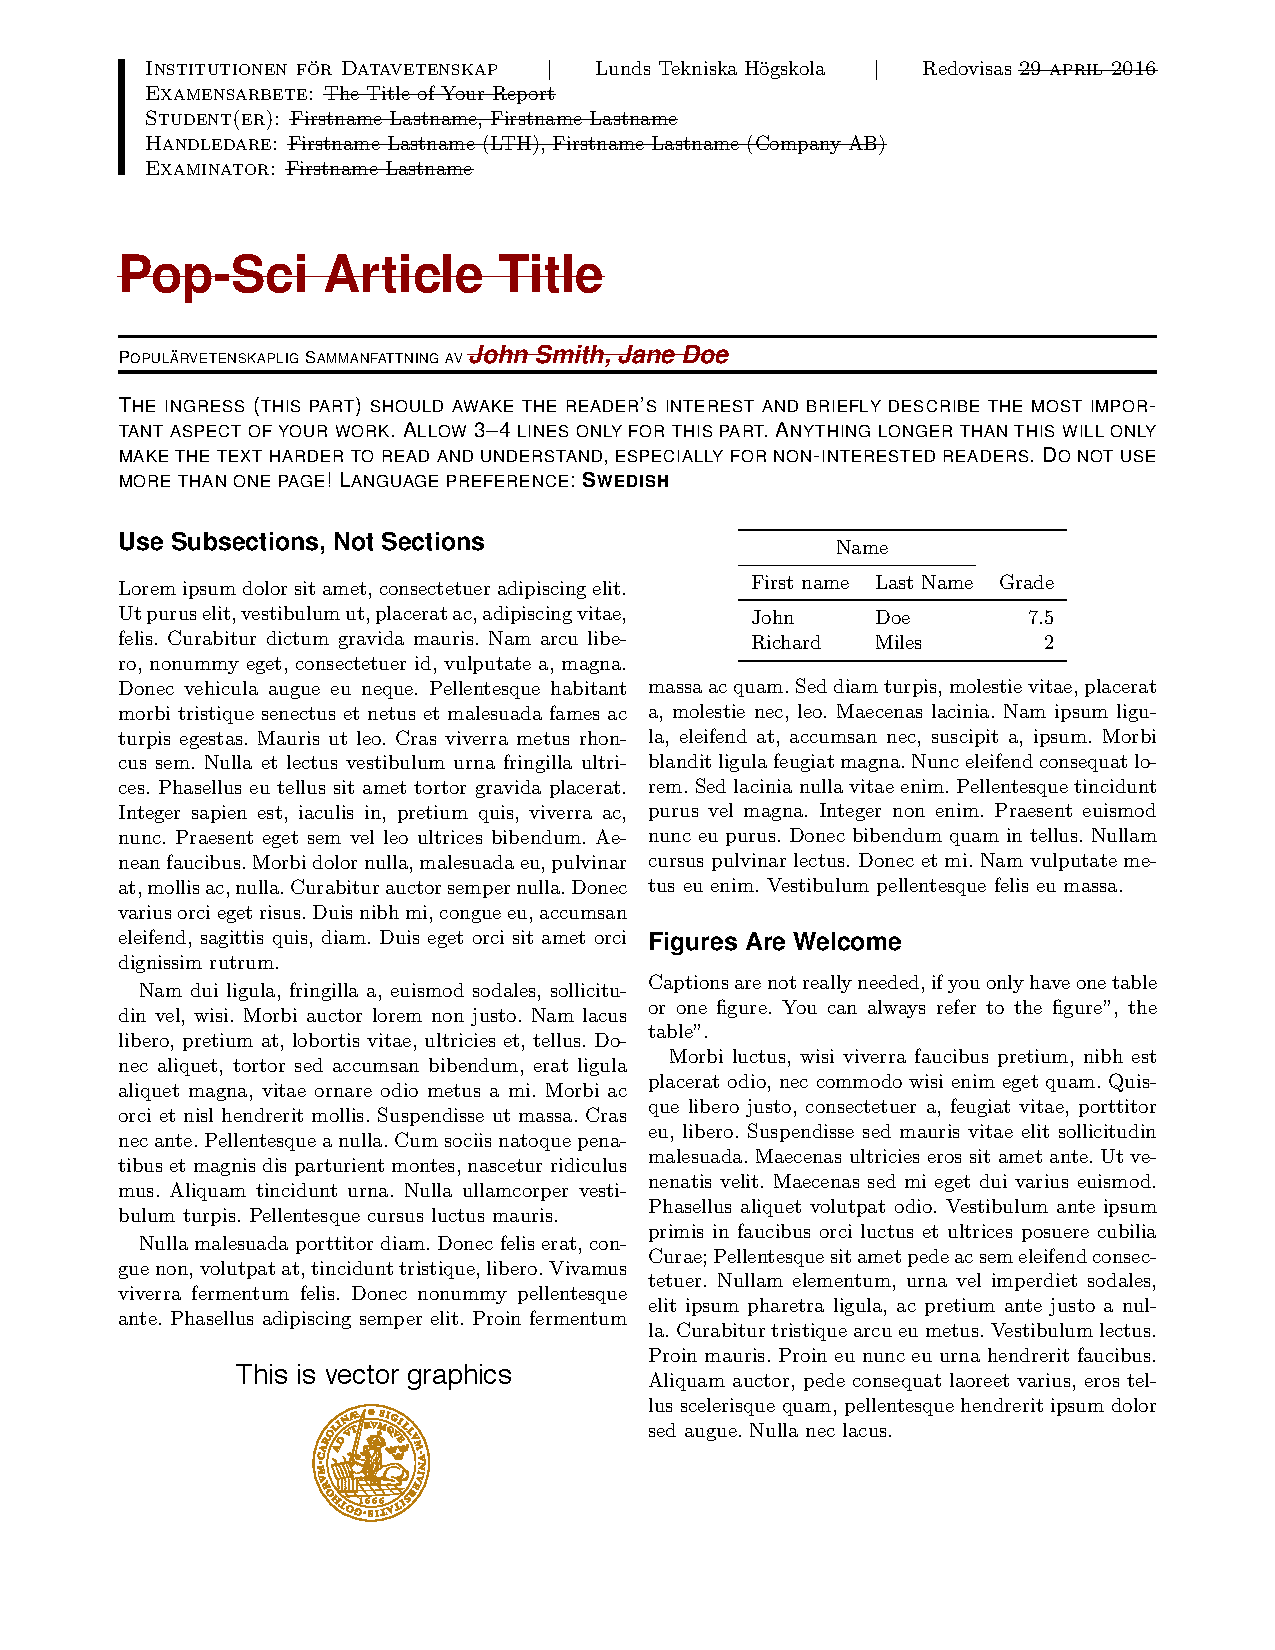
\includepdf[pages={1}]{popsci/popsci.pdf}
\end{appendices}


\end{document}